\documentclass[12pt,a4paper]{article} 
\usepackage[utf8]{inputenx} 
\usepackage[spanish]{babel} 
\usepackage[left=2cm,right=2cm,top=2cm,bottom=2cm]{geometry}
\usepackage{scrextend}
\usepackage{marvosym}
\usepackage{pifont} % Generación de símbolos especiales
\usepackage{textcomp}
\usepackage{newpxtext}
\usepackage{newpxmath}
\usepackage[T1]{fontenc} % Codificación de salida    
\usepackage{microtype} % Mejoras de microtipografía en la obtención de PDF (sólo para pdflatex)
\usepackage[hyphens]{url} % Para escritura de URL
\urlstyle{sf} % Estilo de URL sin serifas para que tengan un mejor aspecto
\usepackage{tikz}
% Paquetes para obtener un mayor control de las listas
\usepackage{paralist} % Mayor control de listas
\usepackage{multicol} % Elementos en varias columnas
\usepackage[breaklinks]{hyperref}
\usepackage{graphicx}
\usepackage{caption}
\captionsetup[figure]{labelformat=empty}
\author{Julián García Sánchez \and Iván Illán Barraya \and Alejandro Medina Jiménez \and Javier Monescillo Buitrón}
\title{Implementación de un procesador de lenguajes para Autómatas de Moore}
\date{\today}
%%%%%%%%%%%%%%

\begin{document}
	
	\maketitle
	
	\begin{figure}[h]
		\centering
		
\includegraphics[width=0.25
		\linewidth]{img/image004}
		\caption{}
		\label{fig:image004}
	\end{figure}

	\newpage
	\tableofcontents
	\newpage
	
	\section{¿Qué es un autómata de Moore?}
	En Teoría de la computación una \textbf{Máquina de Moore} es un autómata de estados finitos para el cual la salida en un momento dado sólo depende de su estado en ese momento, mientras la transición al siguiente estado depende del estado en que se encuentre y de la entrada introducida.
	El diagrama de estados para una máquina de Moore incluirá una señal de salida para cada estado. \cite{Moore1}
	
	\begin{figure}[h]
		\centering
		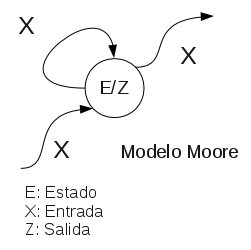
\includegraphics[width=0.5
		\linewidth]{img/Modelo-moore}
		\caption{Ejemplo de Máquina de Moore simple}
		\label{fig:modelo-moore}
	\end{figure}
	
	
	
	El nombre de \textbf{Máquina de Moore} viene de su promotor Edward F. Moore, un pionero de las máquinas de estados, quien escribió \textit{Gedanken-experiments on Sequential Machines,} pp 129-153, Estudios de Autómatas, Anuales de los Estudios Matemáticos, no. 34, Princenton Universityy Press, Princenton, N.J., 1956. \cite{Moore1}
	
	\subsection{Definición formal}
	Una máquina de Moore se define como una 6-tupla:
	\[ Mmor = (S,S_{0},\Sigma,\Lambda,T,G)  \]
	donde definimos los siguientes elementos:
	\begin{itemize}
		\item S: es un conjunto finito de estados.
		\item $S_{0}$: es el estado inicial, y además es un elemento de S.
		\item $\Sigma$: un conjunto finito llamado alfabeto de entrada.
		\item $\Lambda$: un conjunto finito llamado el alfabeto de salida.
		\item $T$ : una función de transición $T: S \times \Sigma \rightarrow S$ mapeando un estado y una entrada al siguiente estado.
		\item $G$ función de salida $G : S \rightarrow \Lambda $ mapeando cada estado al alfabeto de salida.
	\end{itemize}
	\clearpage
	\subsection{Ejemplo concreto}
	Se quiere diseñar una máquina de Moore para el control de una piscina, para ello, se requiere de:
	\newline
	\newline
	El alfabeto de entrada $\Sigma$: {(0,1)}	
	\begin{itemize}
		\item 0 indica que se no ha activado el sensor
		\item 1 indica que se ha activado el sensor
	\end{itemize}

El alfabeto de salida $\Lambda$: {$(Q,F,S,G)$ donde $Q_{i}, F_{i},S_{i},G_{i}\epsilon$ (0,1) }
	\begin{itemize}
		\item $Q:$ se activa el sensor se echa químico en la piscina.
		\item $F:$ se activa el sensor y se calienta la piscina.
		\item $S:$ se activa el sensor y se limpia la piscina.
		\item $G:$ se activa el sensor si detecta una persona.
	\end{itemize}
	
	
	\begin{center}
			
			\textit{Ejemplo del autómata representativo}
	\end{center}
	
	\begin{center}
		\begin{tikzpicture}[scale=0.2]
		\tikzstyle{every node}+=[inner sep=0pt]
		\draw [black] (17,-18.7) circle (3);
		\draw (17,-18.7) node {$q_1/0000$};
		\draw [black] (35.7,-30.1) circle (3);
		\draw (35.7,-30.1) node {$q_2/0100$};
		\draw [black] (16.4,-30.1) circle (3);
		\draw (16.4,-30.1) node {$q_9/1000$};
		\draw [black] (51.7,-32.7) circle (3);
		\draw (51.7,-32.7) node {$q_5/0111$};
		\draw [black] (30.6,-12) circle (3);
		\draw (30.6,-12) node {$q_2/0001$};
		\draw [black] (40.6,-12) circle (3);
		\draw (40.6,-12) node {$q_3/0011$};
		\draw [black] (39.5,-47.6) circle (3);
		\draw (39.5,-47.6) node {$q_4/0101$};
		\draw [black] (51.7,-19.9) circle (3);
		\draw (51.7,-19.9) node {$q_6/0110$};
		\draw [black] (10.1,-39.9) circle (3);
		\draw (10.1,-39.9) node {$q_8/1010$};
		\draw [black] (24.9,-43.1) circle (3);
		\draw (24.9,-43.1) node {$q_0$};
		\draw [black] (40.6,-21.7) circle (3);
		\draw (40.6,-21.7) node {$q_9/0010$};
		\draw [black] (19.56,-20.26) -- (33.14,-28.54);
		\fill [black] (33.14,-28.54) -- (32.72,-27.7) -- (32.2,-28.55);
		\draw [black] (33.14,-28.54) -- (19.56,-20.26);
		\fill [black] (19.56,-20.26) -- (19.98,-21.1) -- (20.5,-20.25);
		\draw (27.55,-23.9) node [above] {$S$};
		\draw [black] (16.84,-21.7) -- (16.56,-27.1);
		\fill [black] (16.56,-27.1) -- (17.1,-26.33) -- (16.1,-26.28);
		\draw (17.28,-24.42) node [right] {$G$};
		\draw [black] (16.56,-27.1) -- (16.84,-21.7);
		\fill [black] (16.84,-21.7) -- (16.3,-22.47) -- (17.3,-22.52);
		\draw [black] (27.91,-13.33) -- (19.69,-17.37);
		\fill [black] (19.69,-17.37) -- (20.63,-17.47) -- (20.19,-16.57);
		\draw [black] (19.98,-19.08) -- (37.62,-21.32);
		\fill [black] (37.62,-21.32) -- (36.89,-20.72) -- (36.77,-21.72);
		\draw (29.14,-19.59) node [above] {$F$};
		\draw [black] (40.6,-18.7) -- (40.6,-15);
		\fill [black] (40.6,-15) -- (40.1,-15.8) -- (41.1,-15.8);
		\draw (41.1,-16.85) node [right] {$Q$};
		\draw [black] (37.62,-21.32) -- (19.98,-19.08);
		\fill [black] (19.98,-19.08) -- (20.71,-19.68) -- (20.83,-18.68);
		\draw [black] (19.69,-17.37) -- (27.91,-13.33);
		\fill [black] (27.91,-13.33) -- (26.97,-13.23) -- (27.41,-14.13);
		\draw (25.09,-15.86) node [below] {$G$};
		\draw [black] (33.6,-12) -- (37.6,-12);
		\fill [black] (37.6,-12) -- (36.8,-11.5) -- (36.8,-12.5);
		\draw (35.6,-11.5) node [above] {$F$};
		\draw [black] (37.6,-12) -- (33.6,-12);
		\fill [black] (33.6,-12) -- (34.4,-12.5) -- (34.4,-11.5);
		\draw [black] (42.02,-14.64) -- (50.28,-30.06);
		\fill [black] (50.28,-30.06) -- (50.34,-29.11) -- (49.46,-29.59);
		\draw (45.47,-23.52) node [left] {$S$};
		\draw [black] (41.4,-45.28) -- (49.8,-35.02);
		\fill [black] (49.8,-35.02) -- (48.91,-35.32) -- (49.68,-35.96);
		\draw (45.04,-38.72) node [left] {$F$};
		\draw [black] (49.8,-35.02) -- (41.4,-45.28);
		\fill [black] (41.4,-45.28) -- (42.29,-44.98) -- (41.52,-44.34);
		\draw [black] (36.751,-48.774) arc (-75.33488:-138.92572:10.168);
		\fill [black] (36.75,-48.77) -- (35.85,-48.49) -- (36.1,-49.46);
		\draw (28.54,-49.3) node [below] {$0101$};
		\draw [black] (27.7,-42.01) -- (48.9,-33.79);
		\fill [black] (48.9,-33.79) -- (47.98,-33.61) -- (48.34,-34.54);
		\draw (41.24,-38.46) node [below] {$0111$};
		\draw [black] (26.059,-40.333) arc (156.89352:149.53508:224.818);
		\fill [black] (39.06,-14.58) -- (38.23,-15.01) -- (39.09,-15.52);
		\draw (31.45,-26.13) node [left] {$0011$};
		\draw [black] (26.82,-40.79) -- (33.78,-32.41);
		\fill [black] (33.78,-32.41) -- (32.89,-32.7) -- (33.66,-33.34);
		\draw (30.85,-38.04) node [right] {$0100$};
		\draw [black] (43.56,-21.22) -- (48.74,-20.38);
		\fill [black] (48.74,-20.38) -- (47.87,-20.01) -- (48.03,-21);
		\draw [black] (48.74,-20.38) -- (43.56,-21.22);
		\fill [black] (43.56,-21.22) -- (44.43,-21.59) -- (44.27,-20.6);
		\draw (45.65,-20.19) node [above] {$F$};
		\draw [black] (14.78,-32.62) -- (11.72,-37.38);
		\fill [black] (11.72,-37.38) -- (12.58,-36.97) -- (11.73,-36.43);
		\draw [black] (11.72,-37.38) -- (14.78,-32.62);
		\fill [black] (14.78,-32.62) -- (13.92,-33.03) -- (14.77,-33.57);
		\draw (13.87,-36.31) node [right] {$F$};
		\draw [black] (18.04,-32.61) -- (23.26,-40.59);
		\fill [black] (23.26,-40.59) -- (23.24,-39.65) -- (22.4,-40.19);
		\draw (21.27,-35.28) node [right] {$Q,S$};
		\draw [black] (25.211,-46.072) arc (33.69737:-254.30263:2.25);
		\draw (20.46,-49.99) node [below] {$Q,S$};
		\fill [black] (22.73,-45.15) -- (21.79,-45.18) -- (22.34,-46.01);
		\draw [black] (13.03,-40.53) -- (21.97,-42.47);
		\fill [black] (21.97,-42.47) -- (21.29,-41.81) -- (21.08,-42.79);
		\draw (16.11,-42.19) node [below] {$Q,S$};
		\draw [black] (51.7,-22.9) -- (51.7,-29.7);
		\fill [black] (51.7,-29.7) -- (52.2,-28.9) -- (51.2,-28.9);
		\draw [black] (51.7,-29.7) -- (51.7,-22.9);
		\fill [black] (51.7,-22.9) -- (51.2,-23.7) -- (52.2,-23.7);
		\draw (52.2,-26.3) node [right] {$Q$};
		\draw [black] (49.431,-21.863) arc (-50.69454:-64.27044:55.159);
		\fill [black] (49.43,-21.86) -- (48.5,-21.98) -- (49.13,-22.76);
		\draw (45.34,-26.19) node [below] {$F$};
		\draw [black] (21.948,-42.594) arc (-105.13324:-275.63853:15.898);
		\fill [black] (27.66,-11.43) -- (26.91,-10.85) -- (26.81,-11.85);
		\draw (9.73,-24.11) node [left] {$0001$};
		\end{tikzpicture}
	\end{center}
	
	
	\newpage
	\subsection{Ejemplo propuesto}
	Definimos una Máquina de Moore para regular el tráfico en el siguiente cruce con los cuatro semáforos:
		
	\begin{figure}[h]
		\centering
		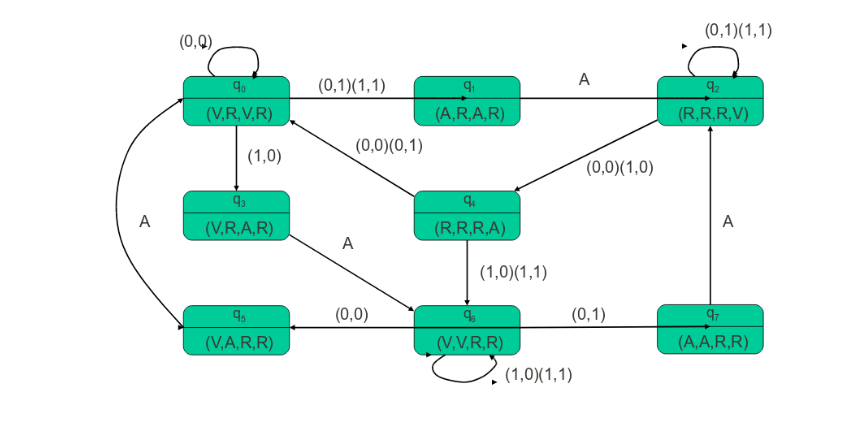
\includegraphics[width=0.4
		\linewidth]{img/4}
		\caption{}
		\label{fig:4}
	\end{figure}

El alfabeto de entrada $\Sigma$: {(0,0),(0,1),(1,0),(1,1)}

	\begin{itemize}
		\item (a,b), donde a es el estado para el sensor $\alpha$ y b para el sensor $\beta$
		\item 0 indica que no hay coches en la cola
		\item 1 indica que hay coches en la cola
	\end{itemize}

El alfabeto de salida $\Lambda$: { ($a_{1},a_{2},a_{3},a_{4}$ donde $a_{i}\epsilon$ (A,V,R) )
	\begin{itemize}
		\item $a_{1}$ es el estado del semáforo 1
		\item $a_{2}$ es el estado del semáforo 2
		\item $a_{3}$ es el estado del semáforo 2
		\item $a_{4}$ es el estado del semáforo 2
	\end{itemize}

	\begin{center}
		\textit{El diagrama de estados sería el siguiente}
	\end{center}

	\begin{figure}[h]
		\centering
		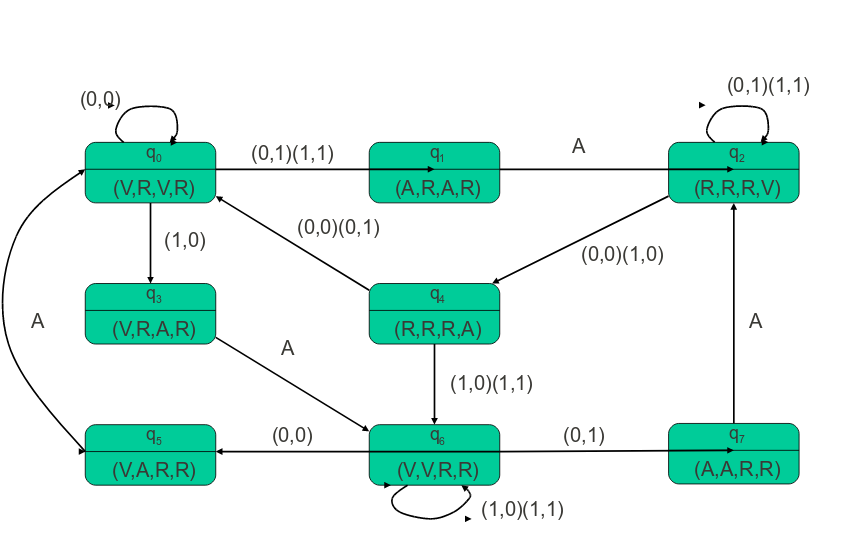
\includegraphics[width=0.7
		\linewidth]{img/3}
		\caption{}
		\label{fig:3}
	\end{figure}

	\newpage
	\section{Presentación del problema}
	\subsection{Lenguaje definido}
	\begin{center}
		\begin{figure}[h]
			\centering
			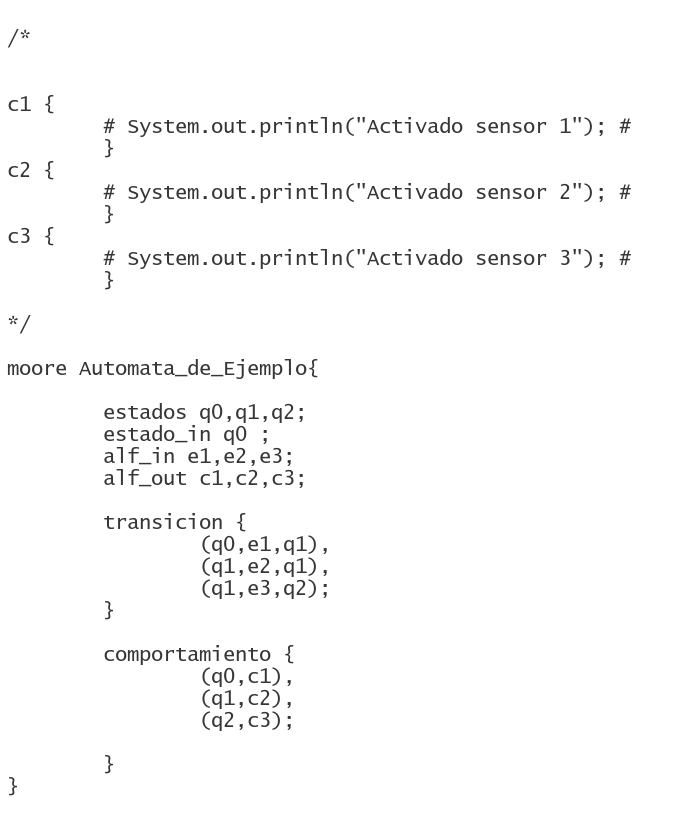
\includegraphics[width=0.7\linewidth]{img/automata2}
			\caption{}
			\label{fig:automata2}
		\end{figure}
	\end{center}
	
	

	\newpage
	\section{EBNF}
			\begin{center}
			\begin{tabular}{|c|c|c|}
				\hline 
		\textbf{Producción izquierda} & ::= & \textbf{Producción derecha} \\ 
				\hline 
				PROGRAMA & ::= & COMP (COMP | AUTOMATA) { AUTOMATA} \\ 
				\hline 
				COMP  &  ::= & $'\ast/'$ DEC$\_$COMP $'\ast/'$ \\ 
				\hline 
				DEC$\_$COMP & ::= & CMP $'\{'$ CODIGO $'\}'$ | $\{$ CMP $'\{'$ CODIGO $'\}'$ $\}$ \\ 
				\hline 
				CODIGO 	& ::=  & '$\#$' ASCII '$\#$' \\ 
				\hline 
				AUTOMATA & ::= & \textbf{moore} ID CUERPO$\_$AUTOMATA \\
				\hline 
			
				CUERPO$\_$AUTOMATA	& ::= & $'\{'$ ESTADOS ESTADO$\_$INI ALF$\_$IN  \\ 
				\hline 
					&  & ALF$\_$OUT TRANSICION COMPORTAMIENTOS $'\}'$ \\ 
				\hline 
				ESTADOS	&  ::= &  \textbf{estados} $\{$ ID ',' $\}$ ID ';'\\ 
				\hline 
				 ESTADO$\_$INI &  ::= & \textbf{estado$\_$in} ID ';'\\ 
				\hline 
				ALF$\_$IN &  ::= & \textbf{alf$\_$in}  $\{$ EVENTOS ',' $\}$ EVENTOS ';' \\ 
				\hline
				ALF$\_$OUT &  ::= & \textbf{alf$\_$out}  $\{$ CMP ',' $\}$ CMP ';'  \\ 
				\hline 
				TRANSICION 	 &  ::= & \textbf{transicion} $'\{'$ TRANSICION$\_$DEF $\{$ TRANSICION$\_$DEF $\}$ $'\}'$ \\ 
				\hline 
				TRANSICION$\_$DEF	 &  ::= & '(' ID ',' EVENTS ',' VAL$\_$TRANS \\ 
				\hline 
				VAL$\_$TRANS &  ::= &  ID ')' ',' | ID ')' ';'\\ 
				\hline 
				COMPORTAMIENTOS	 &  ::= &  \textbf{comportamientos} $'\{'$ COMP$\_$DEF $\{$ COMP$\_$DEF $\}$ $'\}'$\\ 
				\hline 
				COMP$\_$DEF &  ::= & '(' ID ',' VAL$\_$COMP \\ 
				\hline 
				VAL$\_$COMP &  ::= &  CMP ')' ';' | CMP ')' ';' \\ 
				\hline 
				CMP  &  ::= & 'c'NUMEROS \\ 
				\hline 
				 EVENTOS &  ::= & 'e'NUMEROS \\ 
				 \hline 
				 NUMEROS &  ::= & 0 | 1 | .. | 9 \\ 
				 \hline 
				
			\end{tabular} 	
		\end{center}
	
	
	
	

	\newpage
	\section{Tablas de Tokens}
		
	\begin{center}
		\begin{tabular}{|c|c|c|}
			\hline 
			\textbf{Token} & \textbf{Lexema} & \textbf{Patrón} \\ 
			\hline 
			moore & moore & m$\cdot$o$\cdot$o$\cdot$r$\cdot$e  \\ 
			\hline 
			estados &estados & e$\cdot$s$\cdot$t$\cdot$a$\cdot$d$\cdot$o$\cdot$s \\ 
			\hline 
			estado$\_$in & estado$\_$in & e$\cdot$s$\cdot$t$\cdot$a$\cdot$d$\cdot$o$\cdot$$\_$$\cdot$i$\cdot$n \\ 
			\hline 
			alf$\_$in	& alf$\_$in & a$\cdot$l$\cdot$f$\cdot$$\_$i$\cdot$n \\ 
			\hline 
				alf$\_$out	& alf$\_$out & a$\cdot$l$\cdot$f$\cdot$$\_$o$\cdot$u$\cdot$t \\ 
			\hline 
				transicion	& transicion & t$\cdot$r$\cdot$a$\cdot$n$\cdot$s$\cdot$i$\cdot$c$\cdot$i$\cdot$o$\cdot$n \\ 
			\hline 
				comportamiento	& comportamiento & c$\cdot$o$\cdot$m$\cdot$p$\cdot$o$\cdot$r$\cdot$t$\cdot$a$\cdot$m$\cdot$i$\cdot$e$\cdot$n$\cdot$t$\cdot$o \\ 
			\hline 
			Paréntesis abierto	& ( & ( \\ 
			\hline 
			Paréntesis cerrado	& ) & ) \\ 
			\hline 
			Llave abierta	& $\{$ & $\{$ \\ 
			\hline 
			Llave cerrada	& $\}$ & $\}$ \\ 
			\hline 
			Punto y coma	& ; & ; \\ 
			\hline 
			Coma	& , &  , \\ 
			\hline
			Asterisco barra & $\ast/$  & $\ast$$\cdot/$ \\ 
			\hline 
			Barra asterisco & $/\ast$  &  $\ast$$\cdot/$ \\ 
			\hline  
			ID	& hola  & [A-Za-z][A-Zaz0-9$\_$]* \\ 
			\hline 
			CMP	& c1 & c[1-9][0-9]* \\ 
			\hline
			EVENTOS	& e1  & e[1-9][0-9]* \\ 
			\hline
		    CODIGO	& $\#$codigo aquí $\#$  & $\#$$\cdot$ codigo aquí $\cdot$$\#$\\ 
			\hline
		\end{tabular} 	
	\end{center}
	\newpage
	\section{¿Cómo se va a construir el procesador del lenguaje diseñado?}
	\begin{figure}[h]
		\centering
		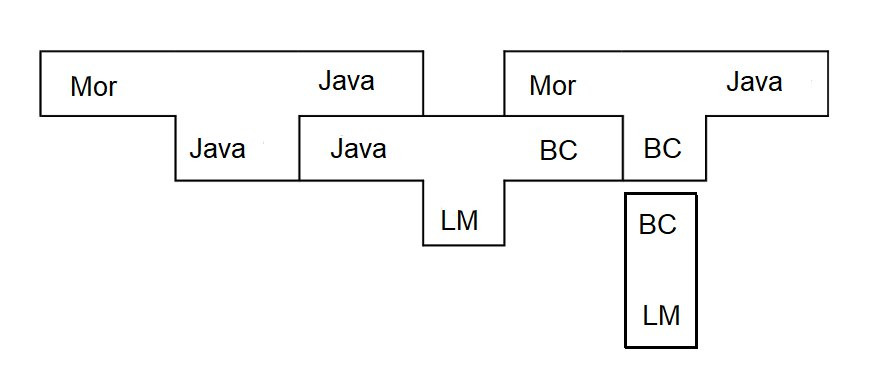
\includegraphics[width=0.7
		\linewidth]{img/photo5978652419892031524}
		\caption{Diagrama tipo T asociado}
		\label{fig:photo5978652419892031524}
	\end{figure}
	
	\newpage
	\begin{thebibliography}{99}
		\bibitem{Moore1} Autómatas de Moore \url{https://es.wikipedia.org/wiki/M%C3%A1quina_de_Moore}
	
	\end{thebibliography}
	
	
	
	
	
\end{document}